\documentclass[12pt,compact]{article}
% \documentclass[main.tex]{subfiles}
\usepackage{amsmath}
\usepackage{graphicx}
\RequirePackage{amsthm,amsmath,multirow,amsfonts,bbm,amssymb,xcolor}
\usepackage{mathtools}  % must be loaded before \DeclarePairedDelimiter
\usepackage[compress]{natbib}
\usepackage{url}

\PassOptionsToPackage{unicode}{hyperref}
\PassOptionsToPackage{hyphens}{url}
\PassOptionsToPackage{dvipsnames,svgnames,x11names}{xcolor}

\usepackage{iftex}
\ifPDFTeX
  \usepackage[T1]{fontenc}
  \usepackage[utf8]{inputenc}
  \usepackage{textcomp} % provide euro and other symbols
\else % if luatex or xetex
  \usepackage{unicode-math}
  \defaultfontfeatures{Scale=MatchLowercase}
  \defaultfontfeatures[\rmfamily]{Ligatures=TeX,Scale=1}
\fi
\usepackage{lmodern}
\ifPDFTeX\else  
    % xetex/luatex font selection
\fi
% Use upquote if available, for straight quotes in verbatim environments
\IfFileExists{upquote.sty}{\usepackage{upquote}}{}
\IfFileExists{microtype.sty}{% use microtype if available
  \usepackage[]{microtype}
  \UseMicrotypeSet[protrusion]{basicmath} % disable protrusion for tt fonts
}{}
\makeatletter
\@ifundefined{KOMAClassName}{% if non-KOMA class
  \IfFileExists{parskip.sty}{%
    \usepackage{parskip} % begin paragraphs with empty line rather than indent
  }{% else
    \setlength{\parindent}{0pt}
    \setlength{\parskip}{6pt plus 2pt minus 1pt}}
}{% if KOMA class
  \KOMAoptions{parskip=half}}
\makeatother
\usepackage{xcolor}
\setlength{\emergencystretch}{3em} % prevent overfull lines
\setcounter{secnumdepth}{5}
% Make \paragraph and \subparagraph free-standing
\makeatletter
\ifx\paragraph\undefined\else
  \let\oldparagraph\paragraph
  \renewcommand{\paragraph}{
    \@ifstar
      \xxxParagraphStar
      \xxxParagraphNoStar
  }
  \newcommand{\xxxParagraphStar}[1]{\oldparagraph*{#1}\mbox{}}
  \newcommand{\xxxParagraphNoStar}[1]{\oldparagraph{#1}\mbox{}}
\fi
\ifx\subparagraph\undefined\else
  \let\oldsubparagraph\subparagraph
  \renewcommand{\subparagraph}{
    \@ifstar
      \xxxSubParagraphStar
      \xxxSubParagraphNoStar
  }
  \newcommand{\xxxSubParagraphStar}[1]{\oldsubparagraph*{#1}\mbox{}}
  \newcommand{\xxxSubParagraphNoStar}[1]{\oldsubparagraph{#1}\mbox{}}
\fi
\makeatother

% NOTE: To produce blinded version, replace "0" with "1" below.
\newcommand{\blind}{0}
\usepackage{rotating}

% DON'T change margins - should be 1 inch all around.
\addtolength{\oddsidemargin}{-.5in}%
\addtolength{\evensidemargin}{-1in}%
\addtolength{\textwidth}{1in}%
\addtolength{\textheight}{1.7in}%
\addtolength{\topmargin}{-1in}%

\newcommand{\red}{\textcolor{red}}

%%%% Non-template packages %%%%
\usepackage{titlesec} % Adjust spacing for sections
\usepackage{tikz}
\usepackage{amsfonts}
\usepackage{natbib} % print author's name and year when citing
\usepackage{bbm}
\usepackage{todonotes}
\usepackage{pdflscape}
\usepackage{caption}
\usepackage{subcaption}
\usepackage{pdfpages}
\usepackage{setspace} 
\usepackage{booktabs}
\usepackage{longtable}
\usepackage{float}
\usepackage{tikz}
\usepackage[colorlinks=true,citecolor=blue, linkcolor=blue]{hyperref}
\usepackage{multirow}
\usepackage{algorithm}
\usepackage{algpseudocode}
\usepackage[defaultlines=2,all]{nowidow} % prevent widows and orphans
\usepackage{enumitem} % inline enumeration
\usepackage{xr-hyper}   % for cross-references that work with hyperref

% external document for cross-referencing
\externaldocument{manuscript_with_author_details}


% penalties for breaking equations
\relpenalty=10000
\binoppenalty=10000

\renewcommand{\theequation}{S.\arabic{equation}}
\renewcommand{\thefigure}{S\arabic{figure}}
\renewcommand{\thesection}{S\arabic{section}}

% Define a custom note command for general notes
\newcommand{\mynote}[1]{\todo[color=yellow!40,inline]{#1}}

% Define custom maths equations 
\DeclareMathOperator{\KL}{KL}
\DeclareMathOperator{\JS}{JS}
\DeclareMathOperator*{\argmin}{arg\,min}
\DeclarePairedDelimiter\abs{\lvert}{\rvert}%
\DeclareMathOperator{\EX}{\mathbb{E}}% expected value
\newcommand{\JSGa}{\mathop{\mathrm{JS}^{\mathrm{G}_{\lambda}}}\nolimits}
\newcommand{\cJSGa}[1]{\mathop{\mathrm{cJS}_{i, #1}^{\mathrm{G}_{\lambda}}}\nolimits}
\newcommand{\eJSGa}[1]{\mathop{\mathrm{eJS}_{i, #1}^{\mathrm{G}_{\lambda}}}\nolimits}
\DeclareRobustCommand{\eJSGai}{\mathop{\mathrm{eJS}^{\mathrm{G}_{\lambda}}}\nolimits}
\DeclareMathOperator{\GJS}{\mathrm{JS}^{\mathrm{G}}}
\DeclareMathOperator{\CE}{\mathrm{CE}}
\newcommand{\rhou}[1]{\rho_{\text{#1}}}
\newcommand\numberthis{\addtocounter{equation}{1}\tag{\theequation}}

\newcommand{\mvmean}[1]{\symbf{\alpha}_{\mid i, #1} y + y^{\symbf{\beta}_{\mid i, #1}} \symbf{\mu}_{\mid i, #1}}
\newcommand{\mvcov}[1]{\left(y^{\symbf{\beta}_{\mid i, #1}}\right)^{\mathrm{T}} \Sigma_{\mid i, #1} y^{\symbf{\beta}_{\mid i, #1}}}

\begin{document}

\def\spacingset#1{\renewcommand{\baselinestretch}%
{#1}\small\normalsize} \spacingset{1}

%%%%%%%%%%%%%%%%%%%%%%%%%%%%%%%%%%%%%%%%%%%%%%%%%%%%%%%%%%%%%%%%%%%%%%%%%%%%%%

\if0\blind
{
  \title{\bf Supplementary material for ``Clustering of multivariate tail dependence using conditional methods''}
  \author{
  Patrick O'Toole\thanks{Patrick O'Toole is supported by a scholarship from the EPSRC Centre for Doctoral Training in Statistical Applied Mathematics at Bath (SAMBa), under the project EP/S022945/1.}\\
  Department of Mathematical Sciences, University of Bath, UK
  \and
  Christian Rohrbeck\\
  Department of Mathematical Sciences, University of Bath, UK 
  \and
  Jordan Richards\\
  School of Mathematics \\
  and Maxwell Institute for Mathematical Sciences, \\
  University of Edinburgh, UK
  }
  \maketitle
} \fi

\if1\blind
{
  \bigskip
  \begin{center}
    {\LARGE\bf Title}
\end{center}
  \medskip
} \fi

\begin{abstract}
  This supplementary materials contains additional plots for the motivating data application in Section~\ref{sec:application} of the main text.
  These include elbow plots for choosing the number of clusters, estimated clusters for $k=2$ and $k=4$, and threshold stability plots for the conditional extremes model fits at five specified locations.
\end{abstract}

\newpage
\spacingset{1.75} % DON'T change the spacing!

% --- Tighter spacing around figures and equations ---
\setlength{\textfloatsep}{10pt plus 1pt minus 2pt}
\setlength{\intextsep}{8pt plus 1pt minus 2pt}
\setlength{\floatsep}{8pt plus 1pt minus 2pt}

\setlength{\abovedisplayskip}{8pt plus 2pt minus 4pt}
\setlength{\belowdisplayskip}{8pt plus 2pt minus 4pt}
\setlength{\abovedisplayshortskip}{4pt plus 2pt minus 4pt}
\setlength{\belowdisplayshortskip}{4pt plus 2pt minus 4pt}

\section{Elbow plots}

Figure~\ref{fig:elbow_plots} gives the ``elbow'' plots of the total within-group sum of squares (TWGSS) against the number of clusters $k$, as described in Section~\ref{subsec:clustering} of the main text, for the motivating data application in Section~\ref{sec:application}.
These are shown for the estimated clusters obtained using the dissimilarity matrix for wind speed conditional on precipitation, precipitation conditional on wind speed, and the aggregated dissimilarity matrix $M$ as described in Equation~\eqref{eq:aggregate_matrix} of the main text.

\begin{figure}[ht]
    \centering
    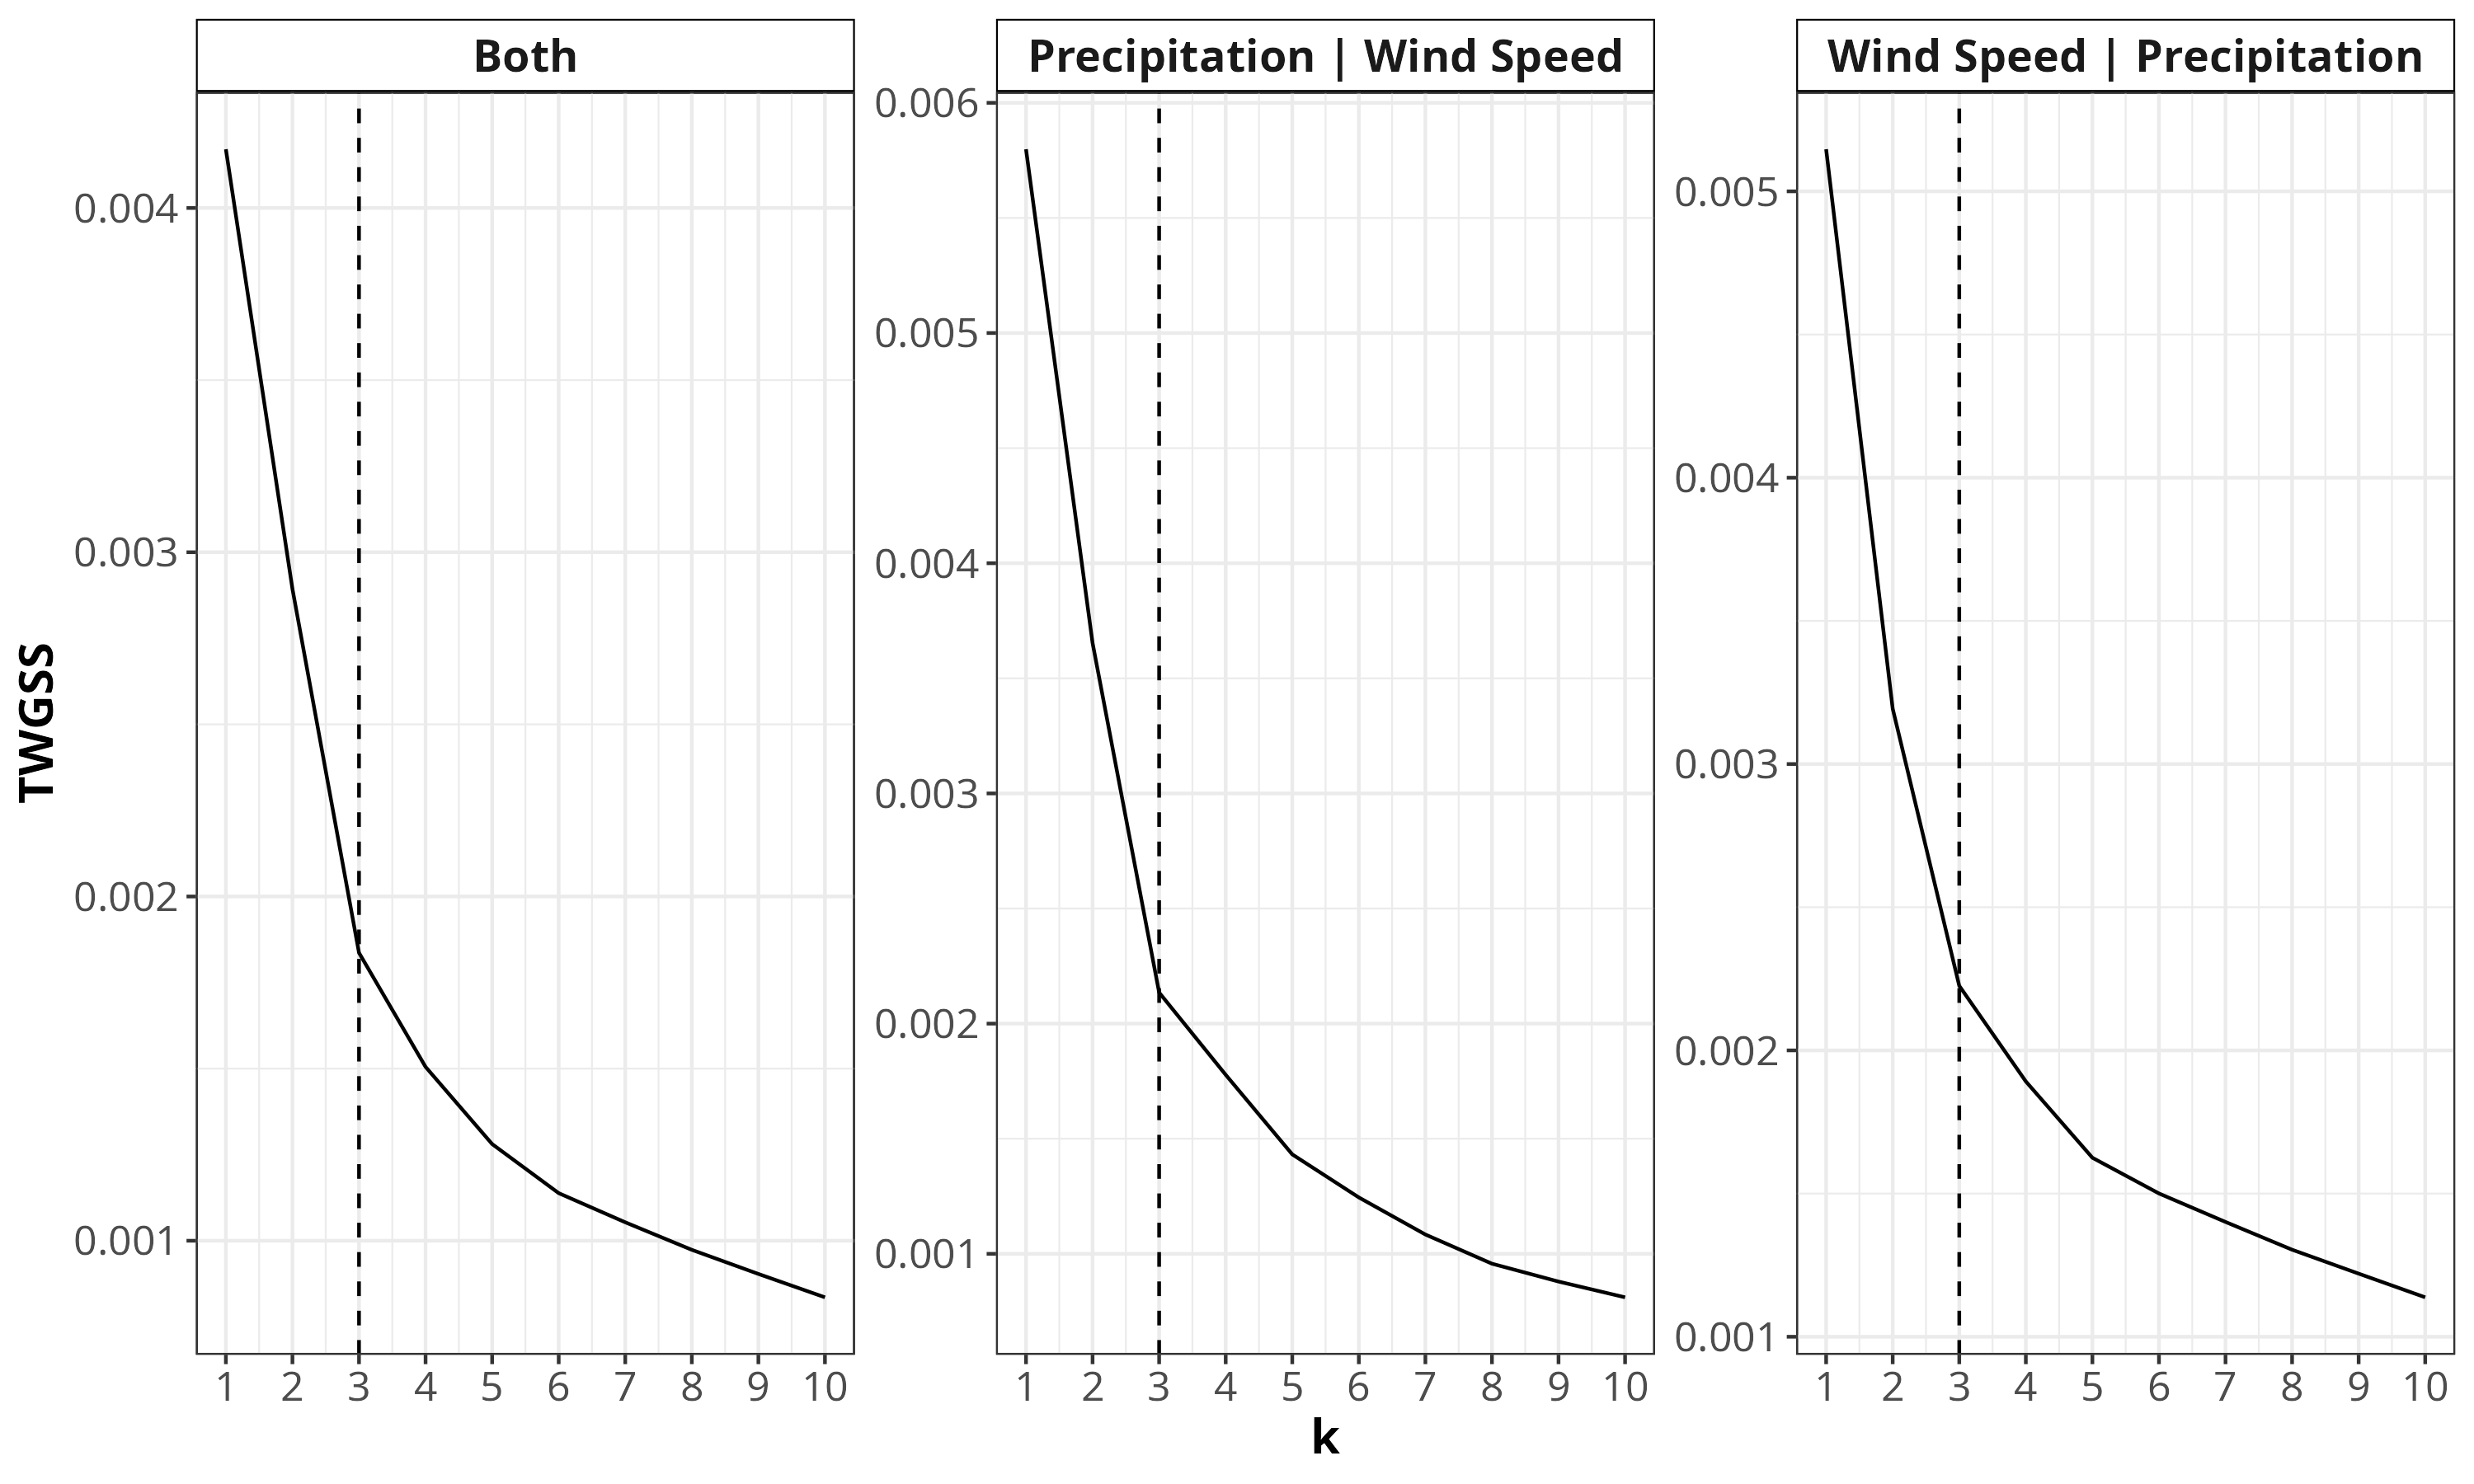
\includegraphics[width = 0.9\linewidth]{plots/cluster_dqu_sep_elbow.png}
    \caption{\emph{ 
      ``Elbow'' plots of the total within-group sum of squares (TWGSS) against the number of clusters $k$ for the estimated clusters obtained using the dissimilarity matrix for wind speed conditional on precipitation (centre), precipitation conditional on wind speed (right), and the combined dissimilarity matrix (left).
    }}
    \label{fig:elbow_plots}
\end{figure}
\clearpage

\section{Estimates for $k=2$ and $k=4$ clusters}

Figure~\ref{fig:cluster_dqu_k_2_4} shows the estimates for $k=2$ and $k=4$ clusters, obtained using the aggregated dissimilarity matrix $M$, as mentioned in Section~\ref{subsec:app_clust} of the main text.

\begin{figure}[ht]
    \centering
    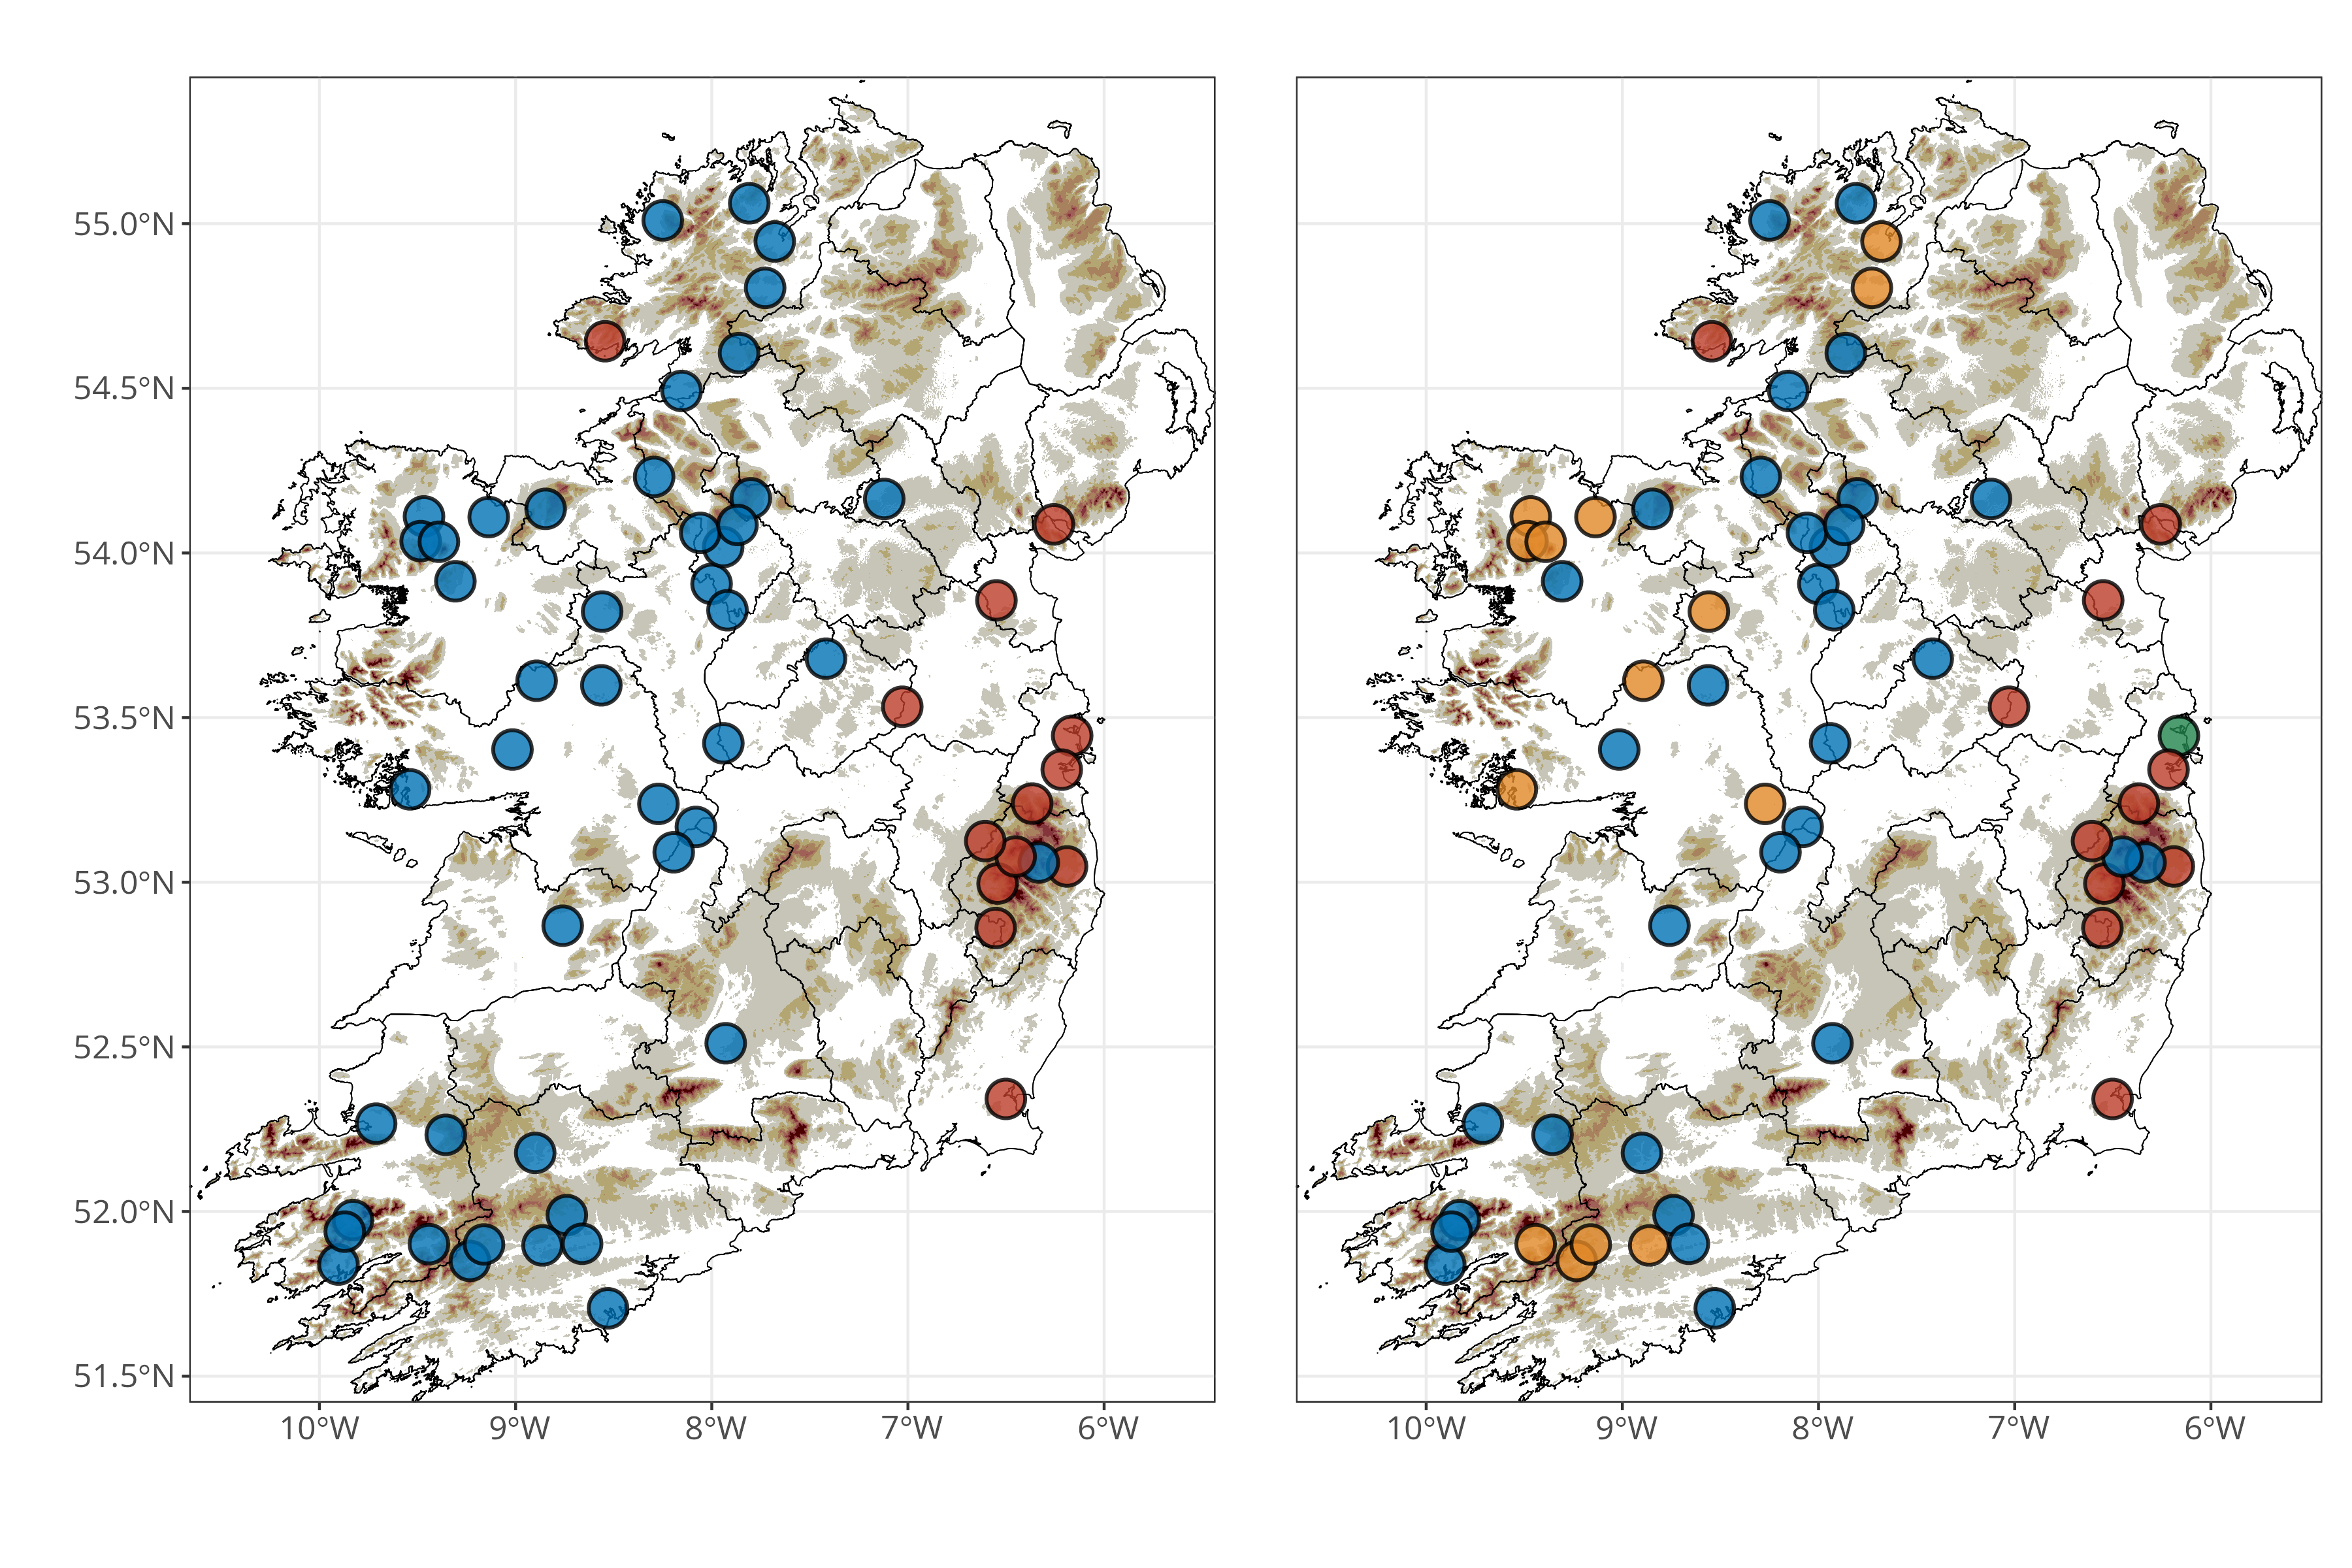
\includegraphics[width = 0.9\linewidth]{plots/cluster_dqu_k_2_4.png}
    \caption{\emph{
    Extremal cluster estimates using the combined dissimilarity matrix for $k = 2$ (left) and $k=4$ (right) clusters. 
    Sites are coloured by cluster label.
    }}
    \label{fig:cluster_dqu_k_2_4}
\end{figure}
\clearpage

\section{Threshold stability plots}

Here, we present threshold stability plots for the conditional extremes model fits at the five locations highlighted in Figure~\ref{fig:chi} of the main text, or specifically, Malahide Castle and Ringsend, both in county Dublin, Glenmacnass in county Wicklow, Kilcar in county Donegal, and Derryhillagh in county Mayo.

\begin{figure}[H]
    \centering
    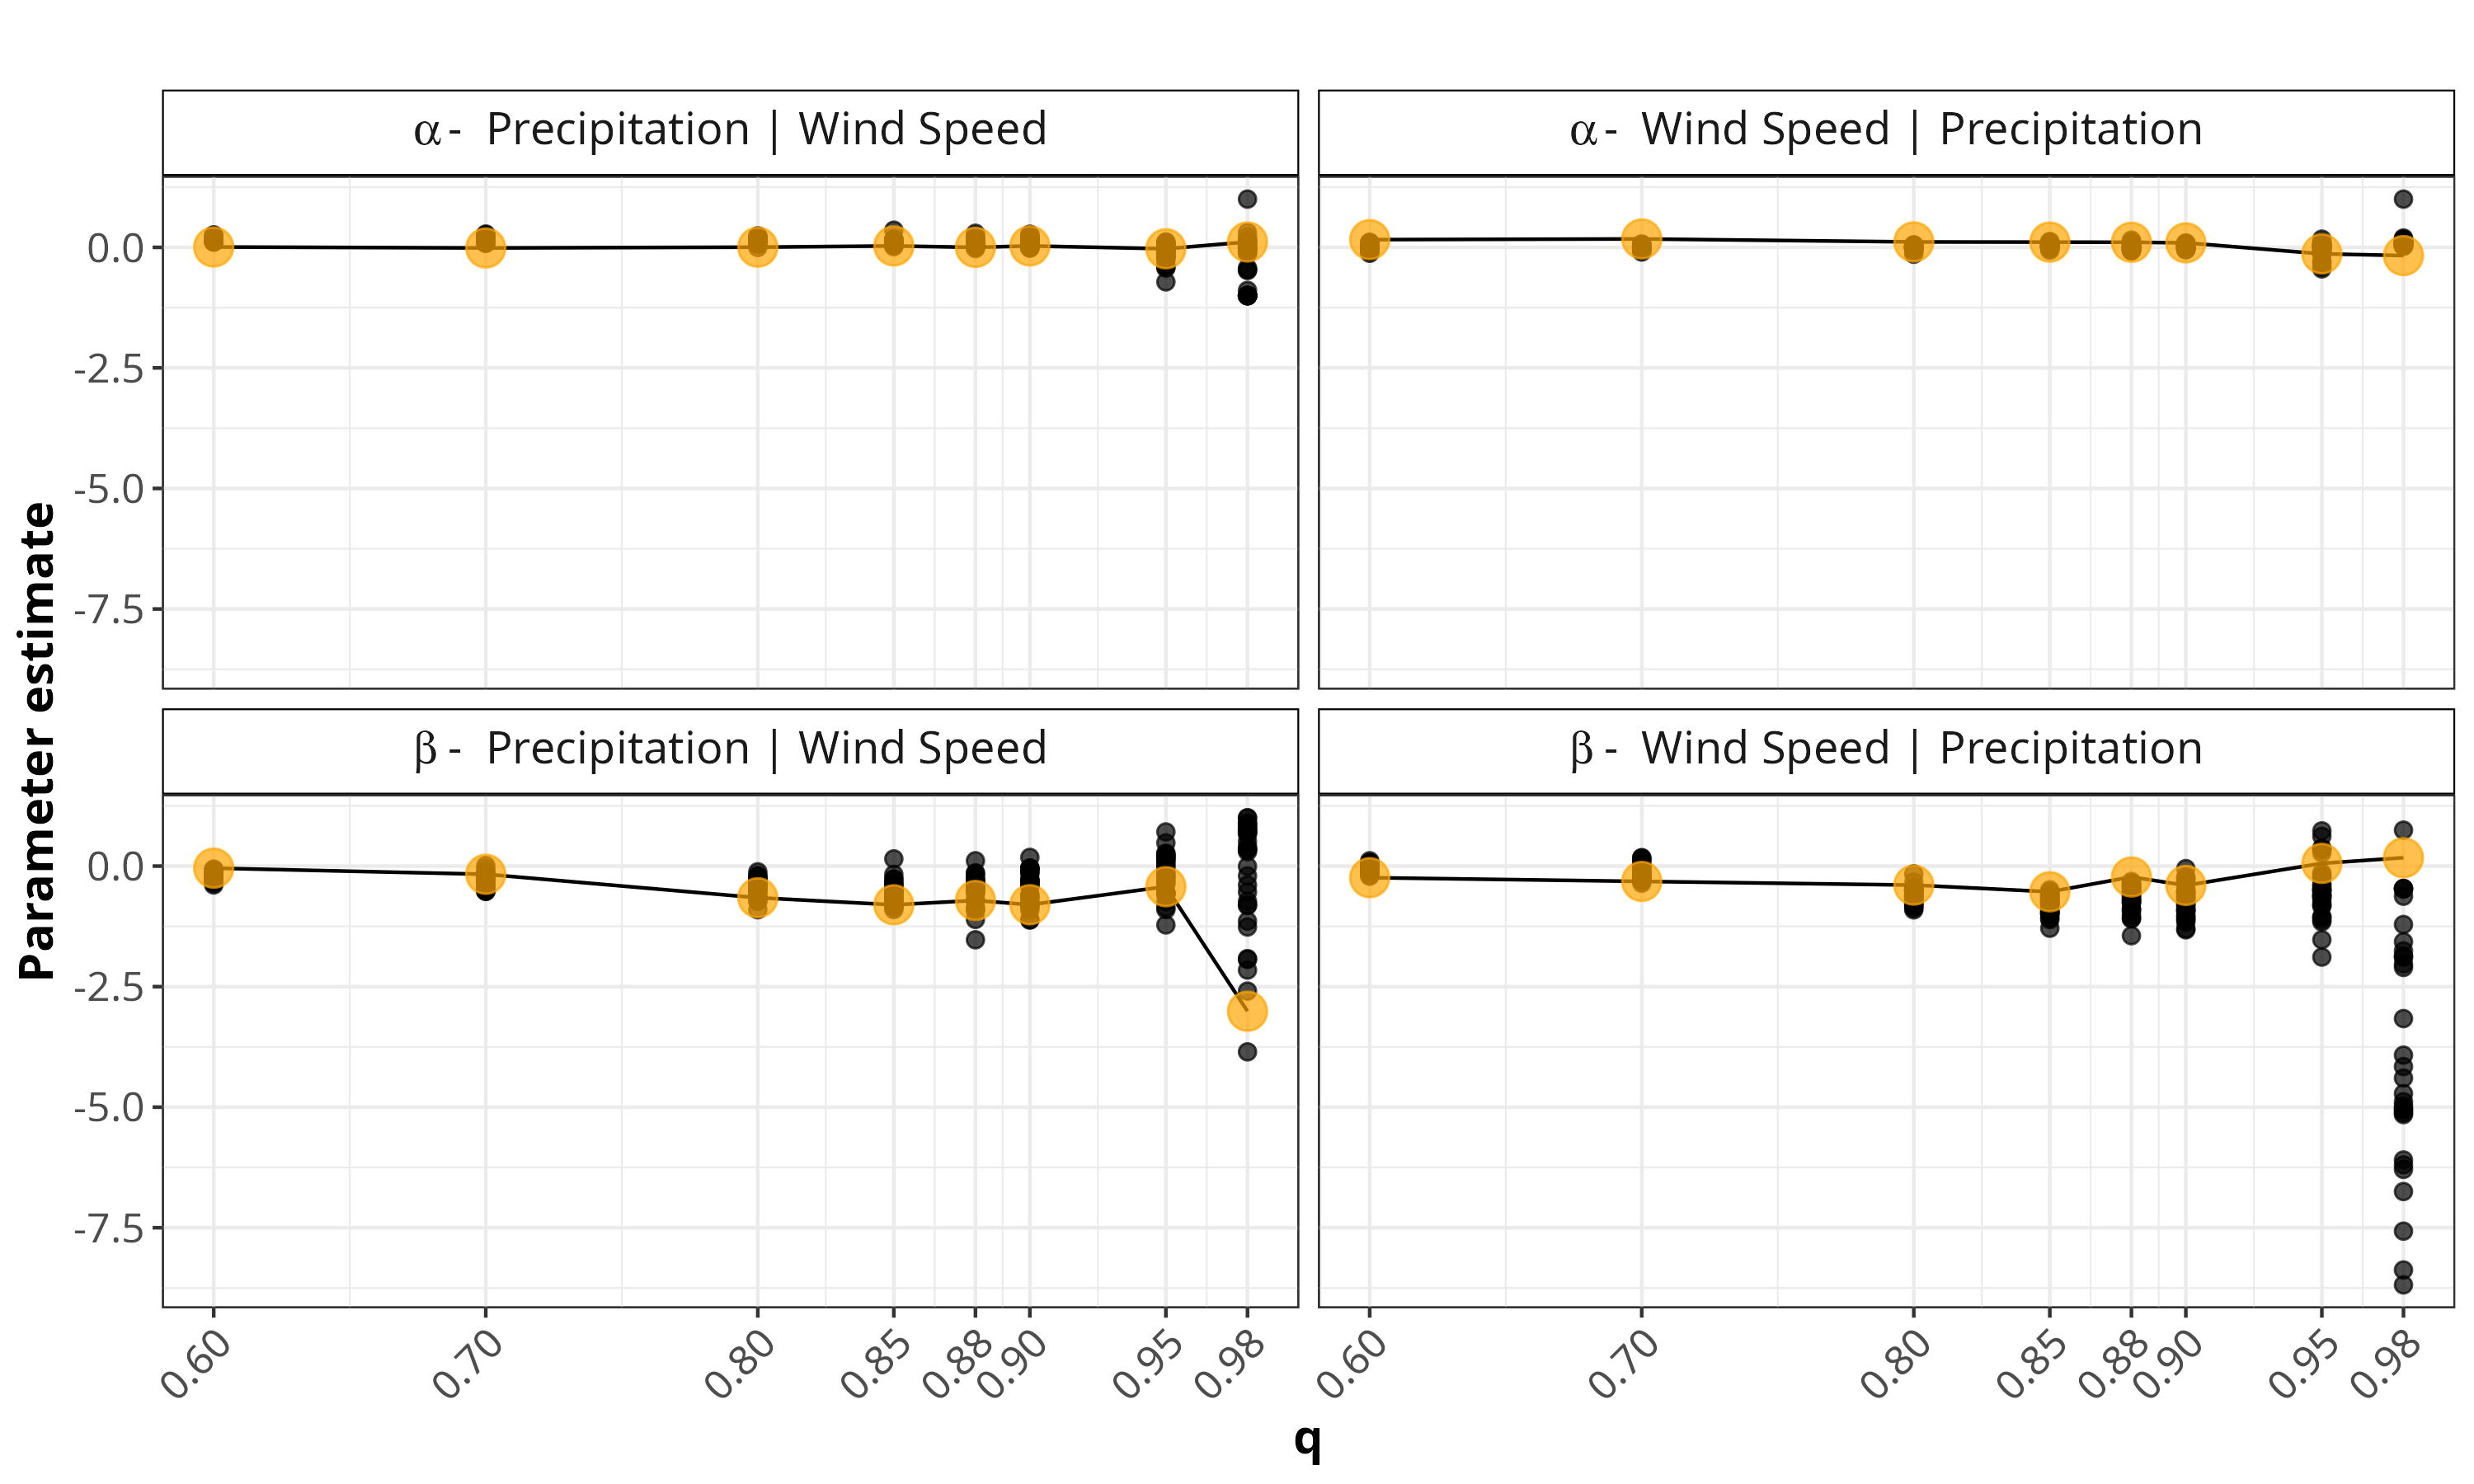
\includegraphics[width = 0.62\linewidth]{plots/boot_quantiles_malahide.png}
    \caption{\emph{
        Threshold stability plots for estimated model parameters $\alpha_{\mid i, s}$ (top) and $\beta_{\mid i, s}$ (bottom) for precipitation conditional on wind speed (left) and wind speed conditional on precipitation (right) at Malahide Castle, county Dublin.
        Estimates for 500 bootstrap samples at each quantile level $q$ of the standard Laplace distribution are shown as black points, with yellow points indicating the estimates obtained using the full data set at each threshold.
    }}
    \label{fig:boot_quantiles_malahide}
\end{figure}

\begin{figure}[H]
    \centering
    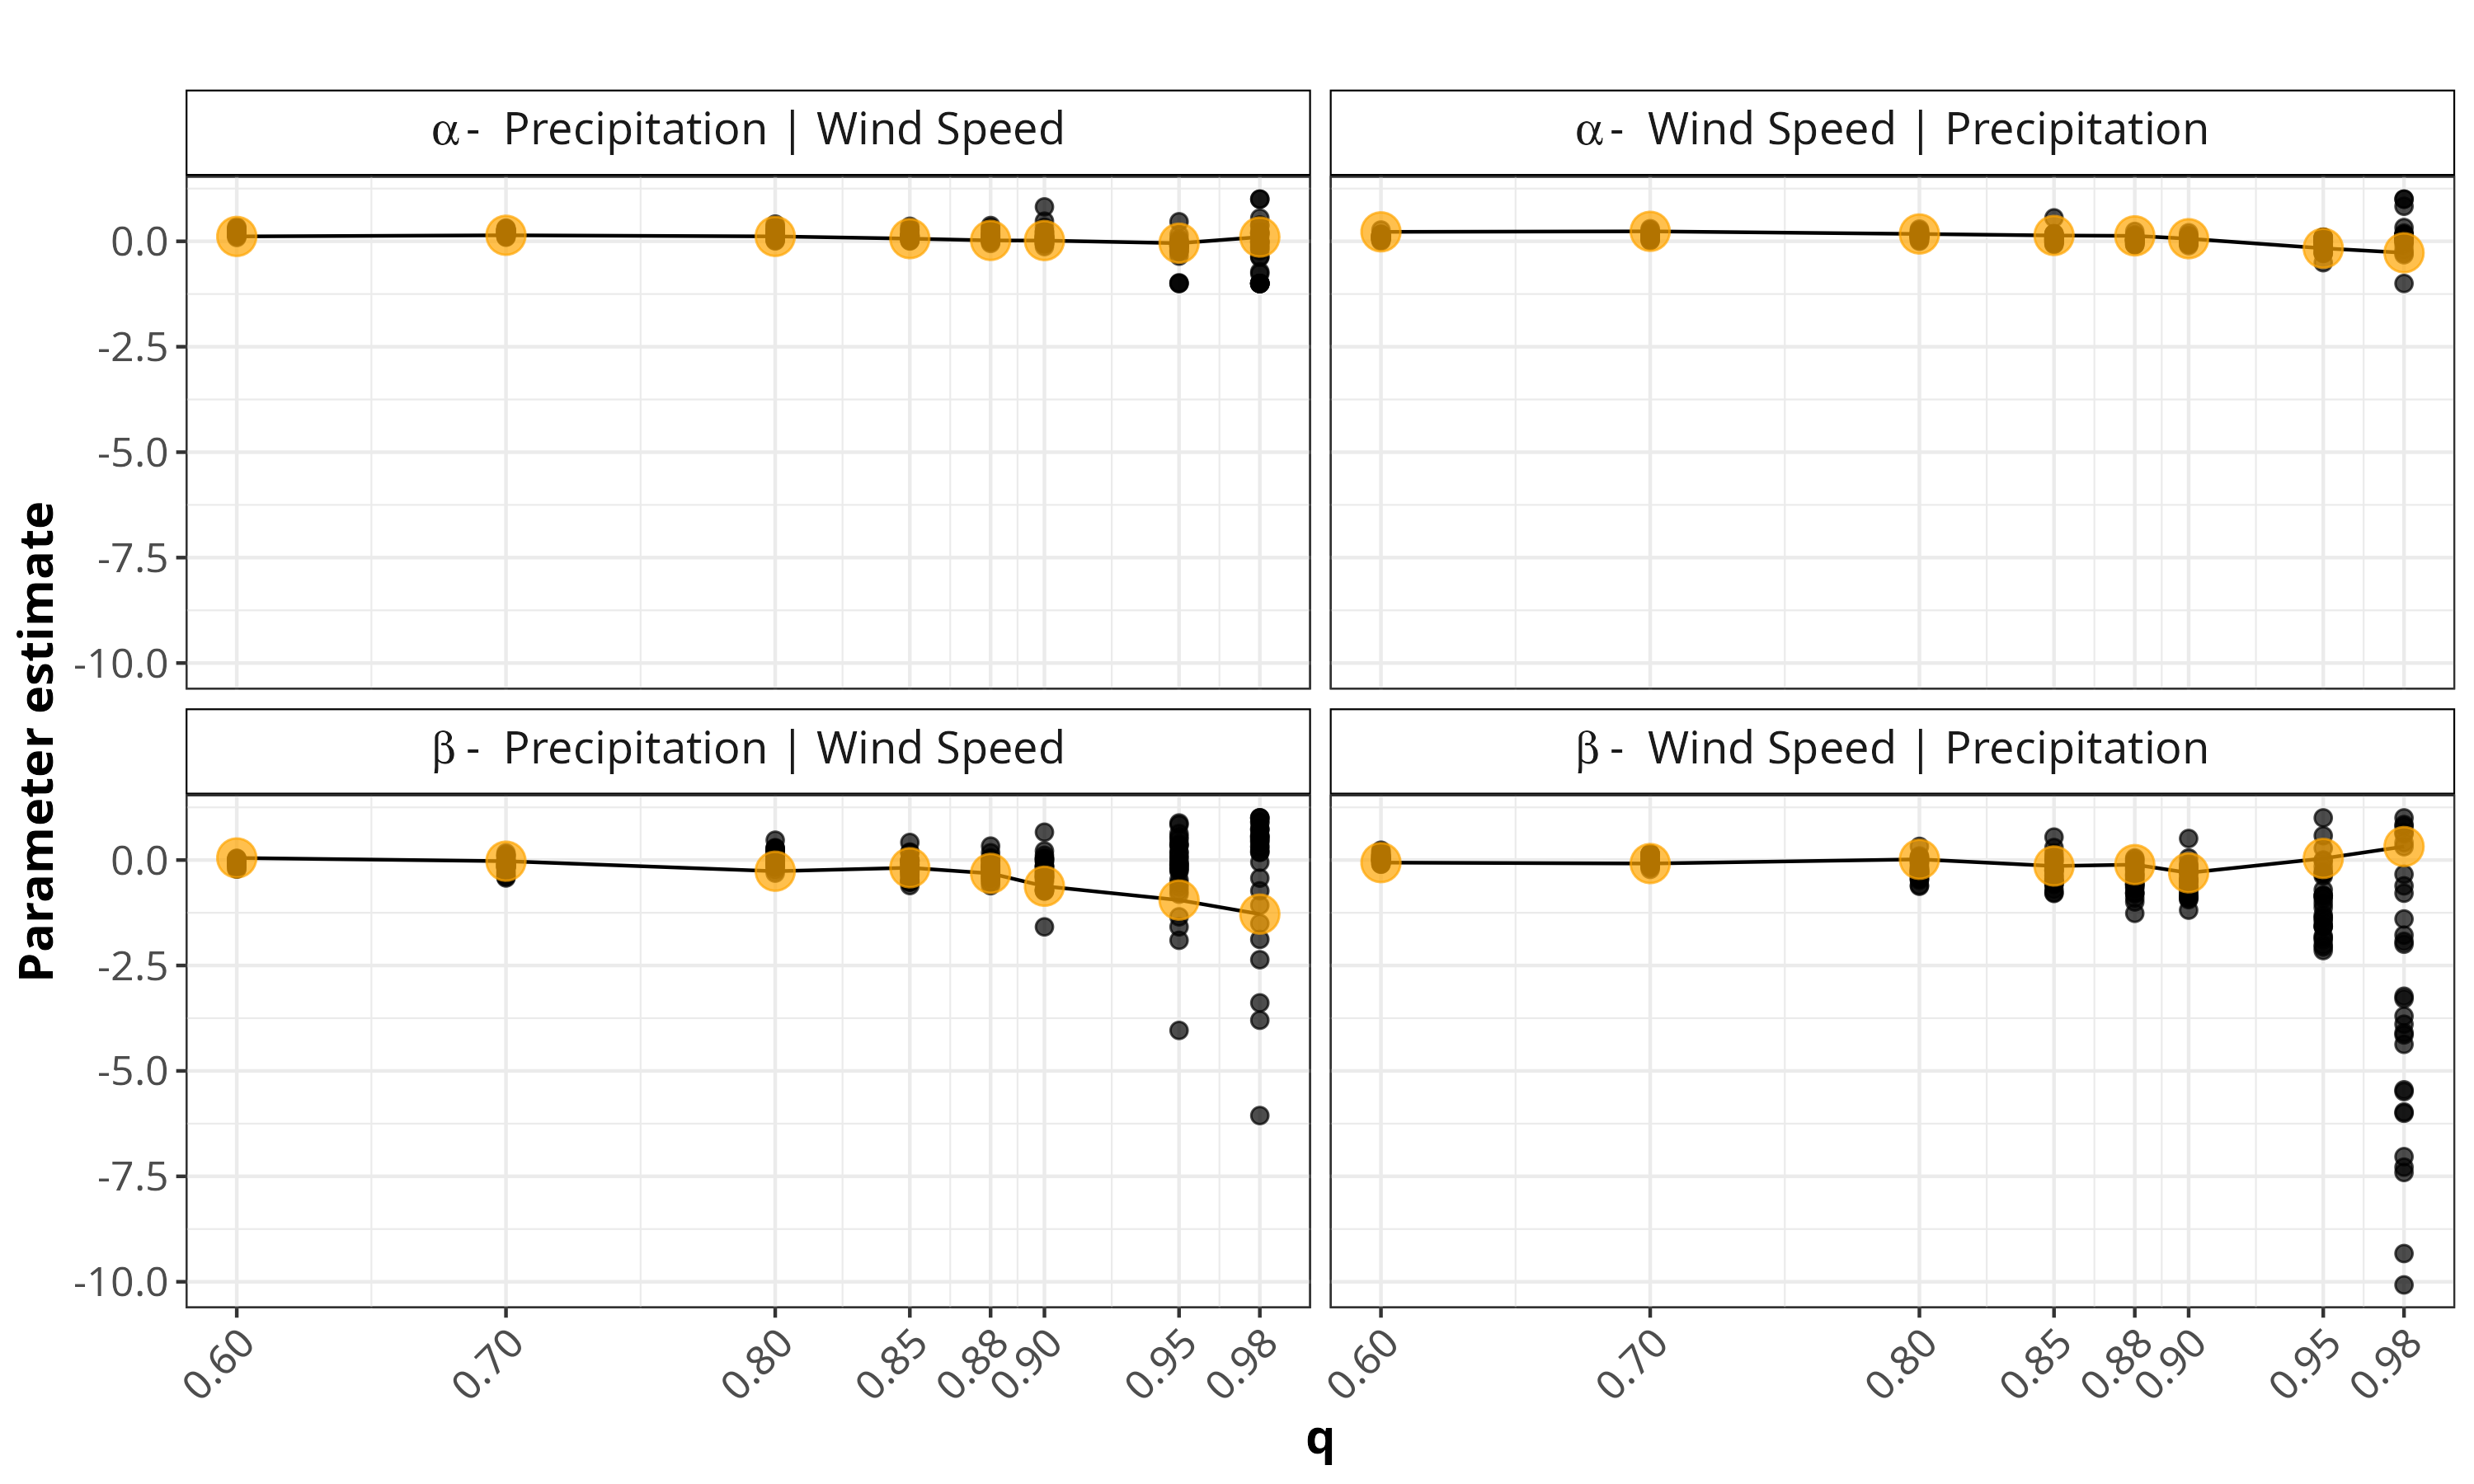
\includegraphics[width = 0.62\linewidth]{plots/boot_quantiles_ringsend.png}
    \caption{\emph{
        Threshold stability plots for estimated model parameters $\alpha_{\mid i, s}$ (top) and $\beta_{\mid i, s}$ (bottom) for precipitation conditional on wind speed (left) and wind speed conditional on precipitation (right) at Ringsend, county Dublin.
        Estimates for 500 bootstrap samples at each quantile level $q$ of the standard Laplace distribution are shown as black points, with yellow points indicating the estimates obtained using the full data set at each threshold.
    }}
    \label{fig:boot_quantiles_ringsend}
\end{figure}

\begin{figure}[H]
    \centering
    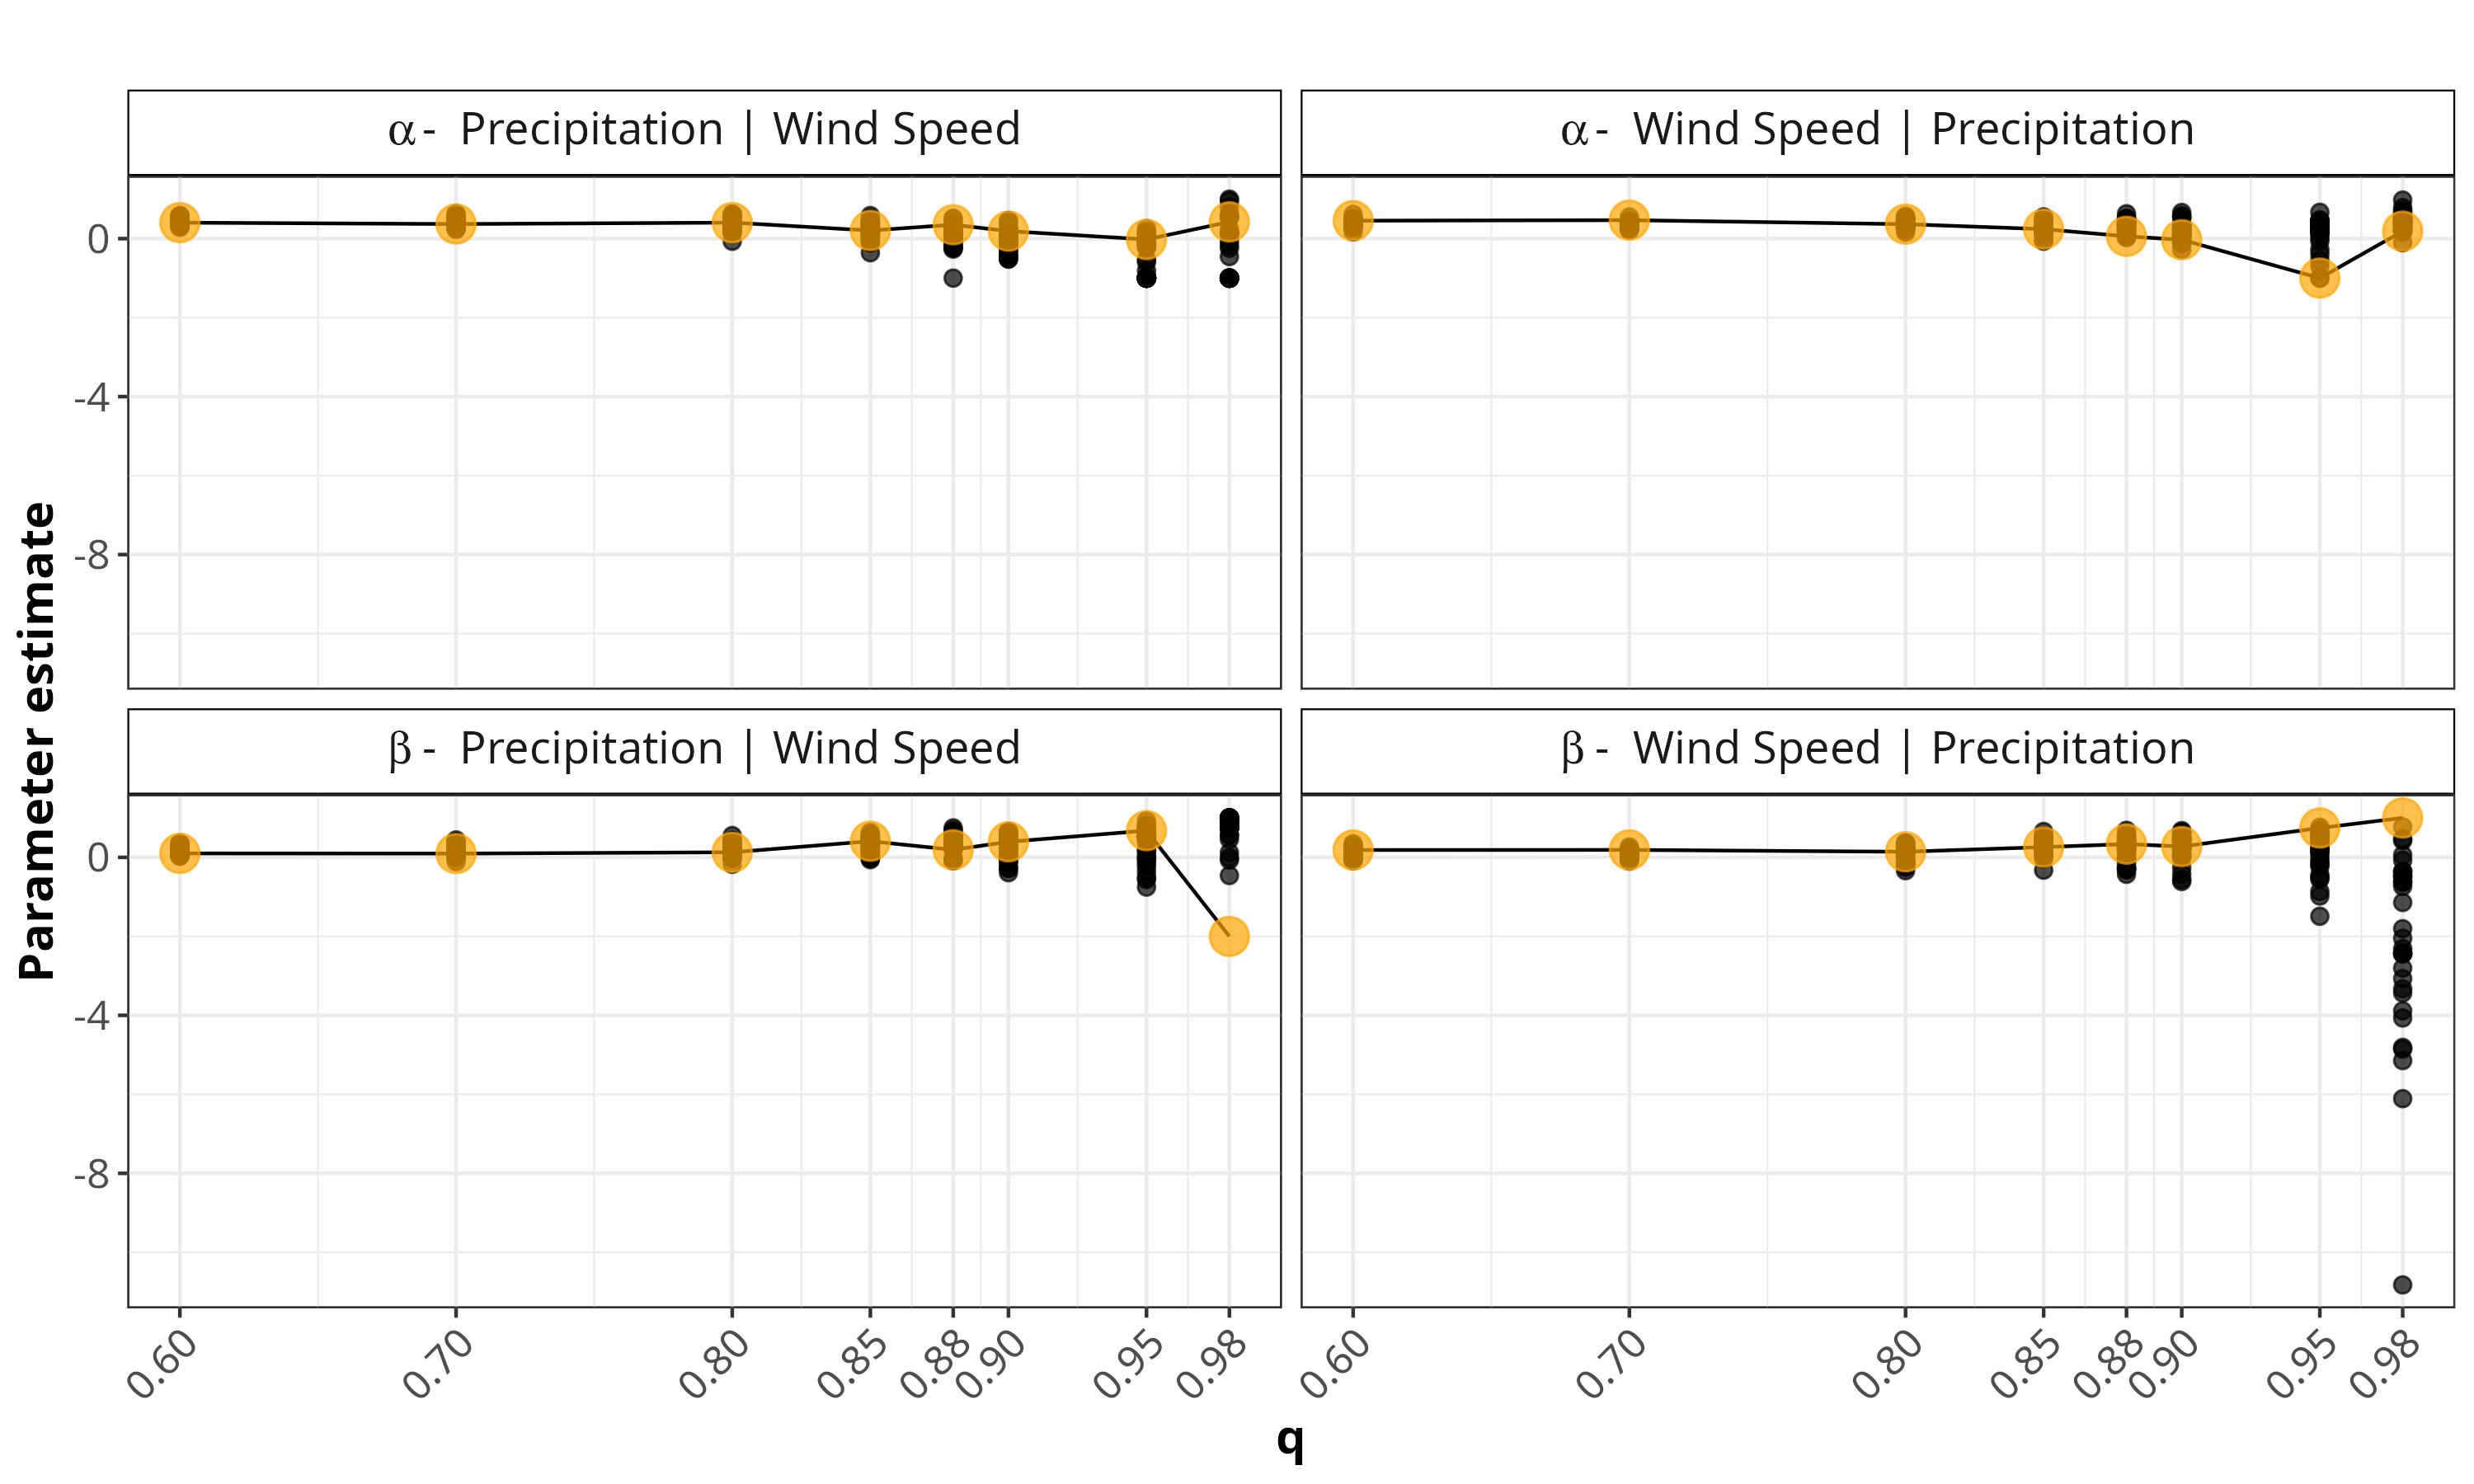
\includegraphics[width = 0.62\linewidth]{plots/boot_quantiles_glenmacnass.png}
    \caption{\emph{
        Threshold stability plots for estimated model parameters $\alpha_{\mid i, s}$ (top) and $\beta_{\mid i, s}$ (bottom) for precipitation conditional on wind speed (left) and wind speed conditional on precipitation (right) at Glenmacnass, county Wicklow.
        Estimates for 500 bootstrap samples at each quantile level $q$ of the standard Laplace distribution are shown as black points, with yellow points indicating the estimates obtained using the full data set at each threshold.
    }}
    \label{fig:boot_quantiles_glenmacnass}
\end{figure}

\begin{figure}[H]
    \centering
    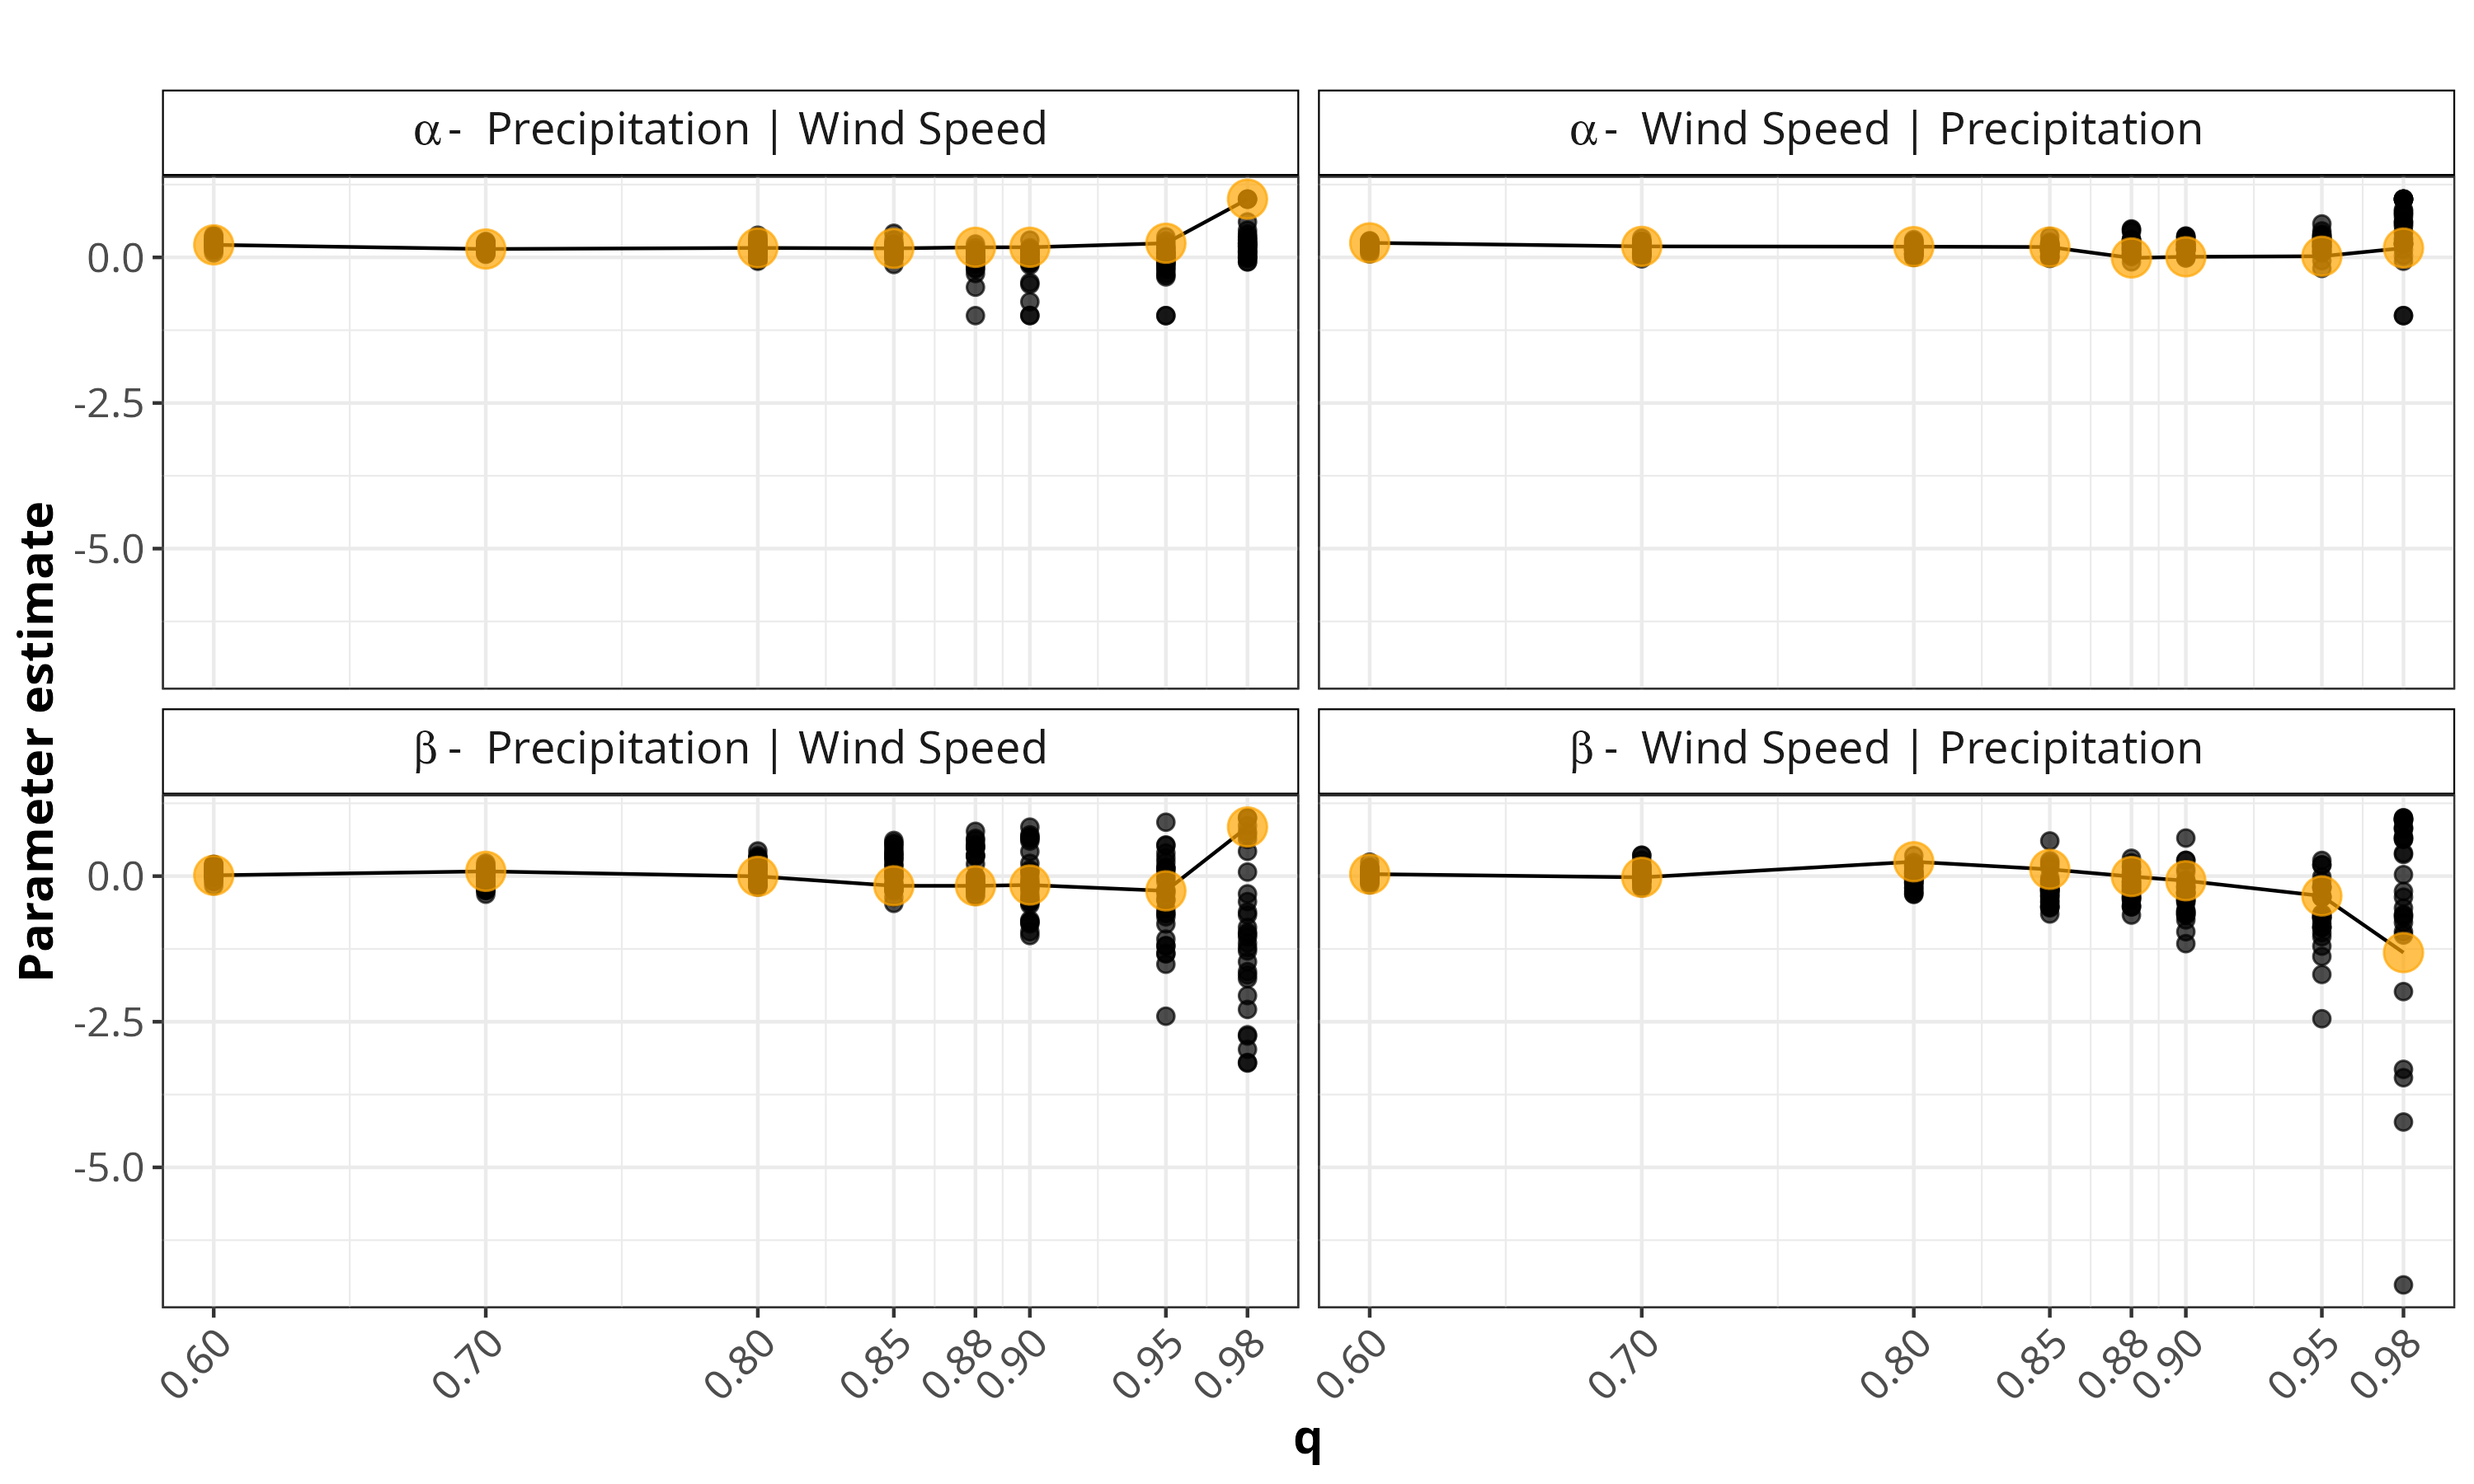
\includegraphics[width = 0.62\linewidth]{plots/boot_quantiles_kilcar.png}
    \caption{\emph{
        Threshold stability plots for estimated model parameters $\alpha_{\mid i, s}$ (top) and $\beta_{\mid i, s}$ (bottom) for precipitation conditional on wind speed (left) and wind speed conditional on precipitation (right) at Kilcar, county Donegal.
        Estimates for 500 bootstrap samples at each quantile level $q$ of the standard Laplace distribution are shown as black points, with yellow points indicating the estimates obtained using the full data set at each threshold.
    }}
    \label{fig:boot_quantiles_kilcar}
\end{figure}

\begin{figure}[H]
    \centering
    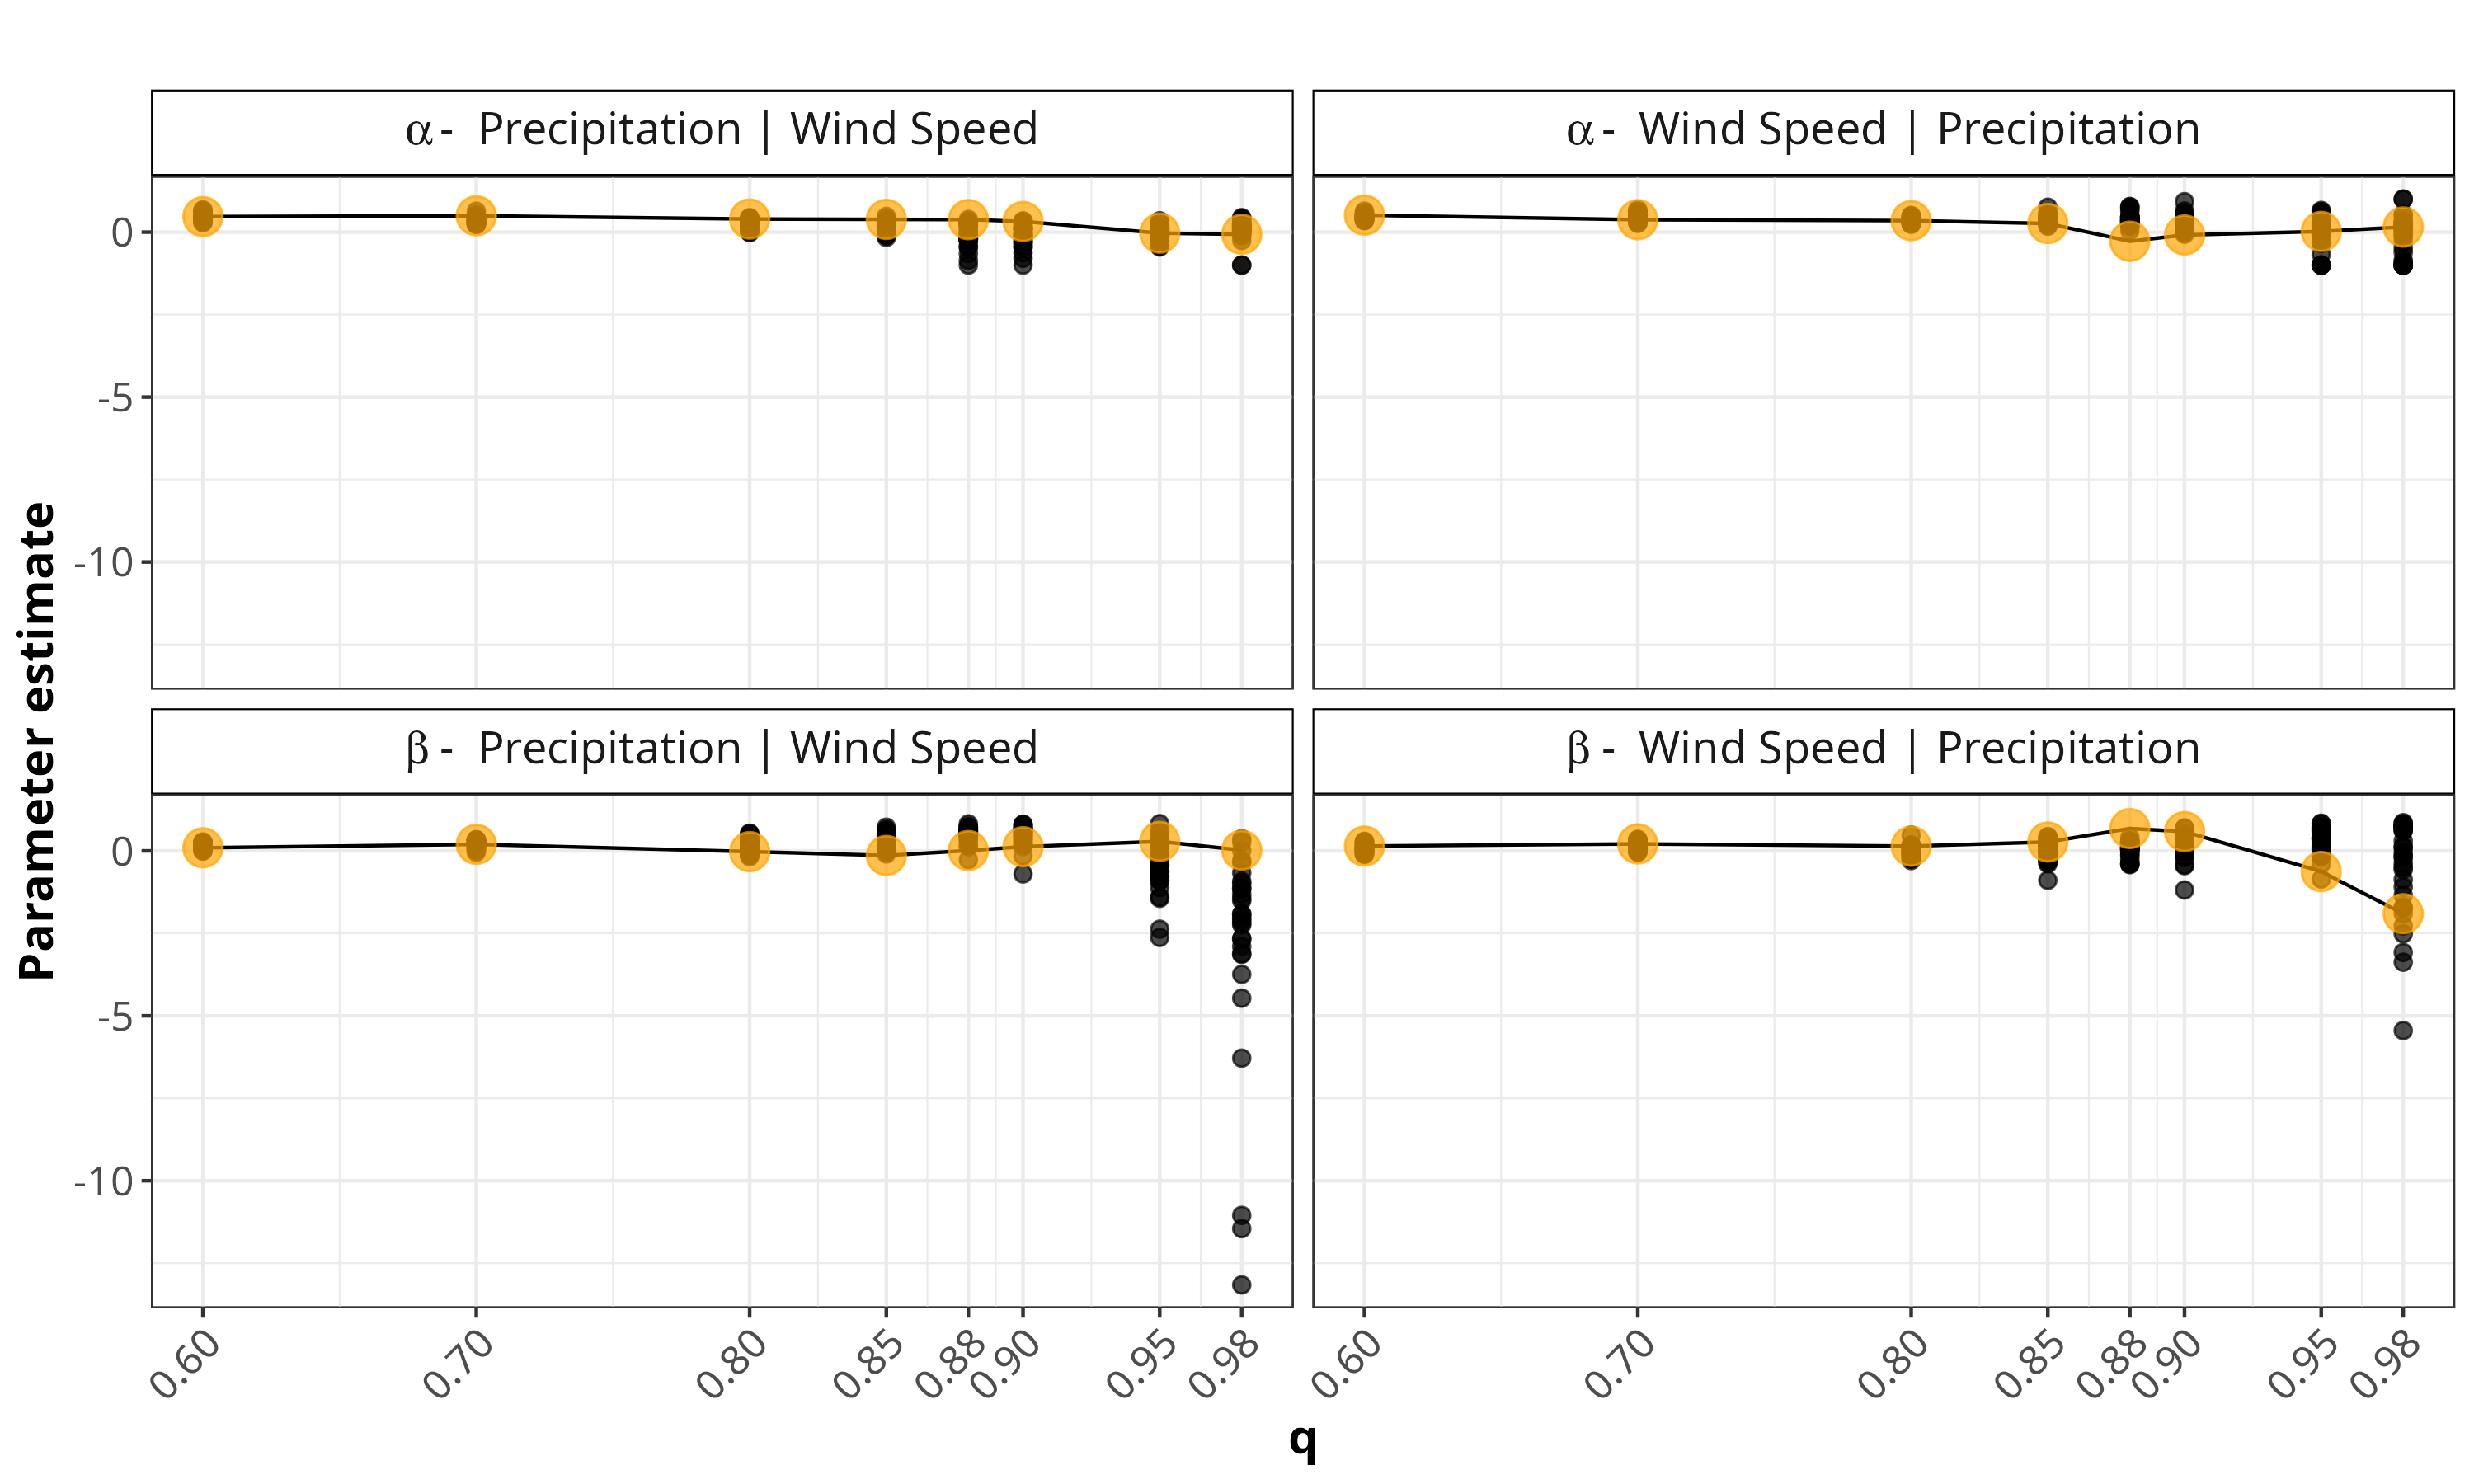
\includegraphics[width = 0.62\linewidth]{plots/boot_quantiles_derryhillagh.png}
    \caption{\emph{
        Threshold stability plots for estimated model parameters $\alpha_{\mid i, s}$ (top) and $\beta_{\mid i, s}$ (bottom) for precipitation conditional on wind speed (left) and wind speed conditional on precipitation (right) at Derryhillagh, county Mayo.
        Estimates for 500 bootstrap samples at each quantile level $q$ of the standard Laplace distribution are shown as black points, with yellow points indicating the estimates obtained using the full data set at each threshold.
    }}
    \label{fig:boot_quantiles_derryhillagh}
\end{figure}

\end{document}
